\chapter{Semesterticket und Ausbildungstarif}

\section{Semesterticket}
Dank des \emph{AK Mobilität zum Semesterticket München} (\url{\http semesterticket-muenchen.de}) hat München nach vielen Jahren nun auch endlich ein Semesterticket für seine Studenten. Bei der Zahlung deines Studienbeitrages ist dir sicherlich aufgefallen, dass du einen Solidarbeitrag in Höhe von 59,00~€ leisten musst. Diesen Beitrag müssen alle Stuika leisten - im Gegenzug darf damit das komplette Netz des MVV befahren werden: täglich von 18-6 Uhr, an Wochenenden und Feiertagen sogar ganztägig.

\begin{figure}[ht]
\centering
\begin{minipage}[b]{0.45\linewidth}
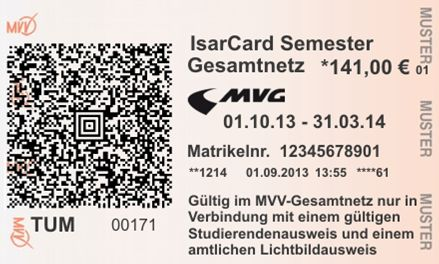
\includegraphics[width=\textwidth]{IsarCardSemester-MVG-ICA-Automat}
\end{minipage}
\quad
\begin{minipage}[b]{0.45\linewidth}
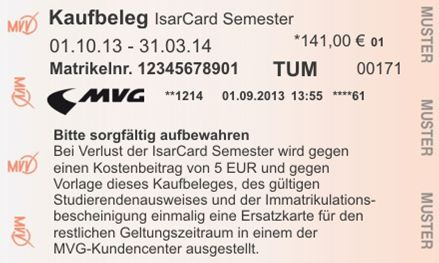
\includegraphics[width=\textwidth]{IsarCardSemester-MVG-ICA-Automat-Kaufbeleg}
\end{minipage}
\end{figure}

Dieser, mit den Vorlesungszeiten inkompatible Gültigkeitsbereich, begründet auch den umgangssprachlichen Titel des "`Partytickets"'.

Möchtest du dein Ticket auch außerhalb dieser Zeiten nutzen, kannst du gegen eine Zahlung von 141,00~€ die Möglichkeit an den Automaten der MVG und der Deutschen Bahn das Semesterticket zu erwerben. Im Gegensatz vom Solidarbeitrag musst du diesen Teil des Tickets aber nicht erwerben, wenn du nicht möchtest bzw. das Ticket nicht brauchst.

Für die meisten Studika, die den MVV nutzen, dürfte das Semesterticket die günstige Möglichkeit sein - es lohnt sich schon, wenn du pro Monat mehr als 23,50~€ in Fahrkarten investieren würdest.

\begin{figure}[ht]
\centering
\begin{minipage}[b]{0.45\linewidth}
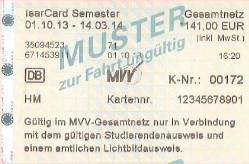
\includegraphics[width=\textwidth]{IsarCardSemester-DB-Automat}
\end{minipage}
\quad
\begin{minipage}[b]{0.45\linewidth}
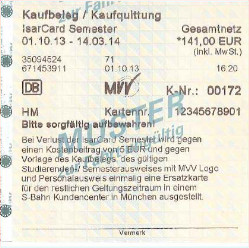
\includegraphics[width=\textwidth]{IsarCardSemester-DB-Automat-Kaufbeleg}
\end{minipage}
\end{figure}

Das Semesterticket - sowohl das "`Partyticket"' als auch der Teil mit Zuzahlung - sind immer für ein Semester gültig. Hier musst du dich auf die auf deinem Studienausweis aufgedruckte Laufzeit des Semesters beziehen - die anderen Hochschulen in München haben teilweise andere Laufzeiten für ihre Semester. Bitte denke auch daran, dass das Semesterticket immer nur zusammen mit deinem Studienausweis gilt, welcher wiederrum nur mit einem amtlichen Ausweisdokument gültig ist.

Wenn du beschließt ein Semesterticket am Automaten zu kaufen (halte bitte deine Matrikelnummer zur Eingabe bereit), erhälts du zwei Belege: Ein Mal das Ticket als solches und einen Zahlungsbeleg. Letzteren solltest du daheim gut aufheben, denn solltest du dein Ticket verlieren, kannst du einmalig gegen Vorlage des Zahlungsbeleges und entrichten von 5,00~€ ein zweites Semesterticket erhalten.

\section{Ausbildungstarif}
Für Studika, die nur sehr selten den MVV in Anspruch nehmen, kann sich unter Umständen auch der vom MVV angebotene Ausbildungstarif II lohnen. Der Preis richtet sich dabei nach der Zahl der benötigten Zeitkartenringe, die befahren werden. Bevor du dir aber ein Ticket kaufen kannst, musst du dir ein Kundenkarte besorgen. Diese bekommst du im MVG-Kundencenter am Hauptbahnhof, Ostbahnhof oder in der Poccistr.~1--3 (alle zwischen 8:00 und 18:00~Uhr). Alternativ kannst du deine Kundenkarte auch direkt online zum selber ausdrucken unter oder online \url{\http mvg-kundenportal.de} beantragen.

Das Ticket gibt es mit der Gültigkeit einer Woche (9,90 -- 40,40~€) oder eines Monats (36,10 -- 147,30~€) an einem der MVG-Zeitkartenautomaten, in den MVG-Kundencentern oder den MVG-Verkaufsstellen. Monatsfahrkarten gelten bis 12Uhr des ersten Werktags des Folgemonats.\\

Mehr Infos zum Ausbildungstarif: \url{\http mvg-mobil.de/tarife/ausbildungstarif.html}